\section {Evaluation}

In this section, we evaluate the performance of the various NFs built with \netstar. Even though future/promise paradigm can simplify asynchronous programming, using this paradigm adds additional overhead to dynamically create special runtime objects (Sec.~\ref{sec:intro-future-promise}). Therefore a natural question to ask is whether the performance of \netstar~is good enough to approach line-rate processing. To answer this question, we design a series of experiments to evaluate the maximum throughput achieved by the \netstar~NFs. We also compare \netstar~with several NFs that are implemented with fast, low-overhead callback-based method to reveal the overhead associated with using future/promise abstraction. The second question involves the effectiveness of future/promise abstraction for simplifying the implementation. To answer this question, we adopt a similar quantitative methodology \cite{syme2011f} used for evaluating F\# future/promise abstraction and compare the required lines of code for implementing the core processing logic between \netstar~NFs and NFs built with callback method.
% for implementing NFs using \netstar and

\subsection {Methodology}

\noindent \textbf{Testbed.} Our testbed consists of 5 servers: three Dell R430 servers, each equipped with one Intel Xeon E5-2650 CPU 2.30GHz with 10 physical cores and 48GB memory, and two Supermicro servers, each with one Intel Xeon E5-1620 CPU 3.50GHz with 4 physical cores and 32GB memory. All servers are equipped with two Intel X710 10Gbps NICs and they are connected through a Dell 10Gbps Ethernet switch. We divide the servers to run our NFs and traffic generators (flow sources and destinations). %Throughout our evaluation, we use one of the Dell R430 server to run our NF application. The rest of the servers are dedicated to traffic generation.

\noindent \textbf{Traffic generation.} We use two types of traffic generators. The first is a custom packet generator that we built on top of \netstar, which can generate 64-bytes UDP/TCP packets at 14Mpps (packets per second), \ie, 10Gbps. The number of flows and the packet size for generation are adjustable. This generator is used to produce flows to NFs such as the packet forwarder (Sec.~\ref{sec:eval1} and Sec.~\ref{sec:eval6}) and the NFs from StatelessNF paper (Sec.~\ref{sec:eval2}). To measure packet processing latency, this generator tags each produced packet with a generation time and computes the packet processing latency by an NF after receiving the packet back from the NF (in this case, source and destination of the flows are the same). The second traffic generator is the default HTTP benchmarking tool provided by Seastar. The tool runs in a client-server setting by sending a large number of HTTP requests from a client and receiving corresponding HTTP responses at the server. We modified this tool, including adding support for HTTP POST method for a client to upload files to the server and recording the HTTP transaction completion time, which is the time interval between sending HTTP request and receiving HTTP response. We use flows produced by this traffic generator to evaluate NFs such as the HTTP reverse proxy (Sec.~\ref{sec:eval3}), the IDS (Sec.~\ref{sec:eval4}) and the malware detector (Sec.~\ref{sec:eval5}).
%eval1 microbench, eval2 stateless nf, eval3 proxy, eval4 ids, eval5 malwares
% eval6 coroutine


\noindent \textbf{Metric.}
We focus on three types of key performance metrics. (1) \textbf{Packet processing throughput} achieved by an NF, measured in the number of processed packets per second (Sec.~\ref{sec:eval1},~\ref{sec:eval2},~\ref{sec:eval6}), the number of processed HTTP requests per second (Sec.~\ref{sec:eval3}) and total bandwidth consumed by all the HTTP connections (Sec.~\ref{sec:eval4}, ~\ref{sec:eval5}).
(2) \textbf{Latency}, computed as average packet processing delay (Sec.~\ref{sec:eval2}) or the average HTTP transaction completion time (Sec.~\ref{sec:eval3},~\ref{sec:eval4},~\ref{sec:eval5}). (3) \textbf{Lines of code (LOC)} for implementing the core packet processing logic, meant for comparing the implementation difficulty using our future/promise based framework and the callback-based asynchronous programming. %(following the approach used in \cite{syme2011f} which uses LOC as the metric to evaluate some future/promise implementation in C\#).

\noindent \textbf{Baselines.} For comparison with NFs implemented using \netstar, we implement various NFs using callback based asynchronous programming (except for HAProxy \cite{haproxy} and TinyProxy \cite{tinyproxy}), following the practice in existing NF implementation.

\subsection{Micro Benchmarking}
\label{sec:eval1}

We first carry out a set of micro benchmarking experiments to evaluate the performance of \netstar~for basic packet processing and asynchronous operations.

\subsubsection{Packet Processing Throughput}

\begin{figure}[!h]
  \begin{subfigure}[t]{0.49\linewidth}
    \centering
    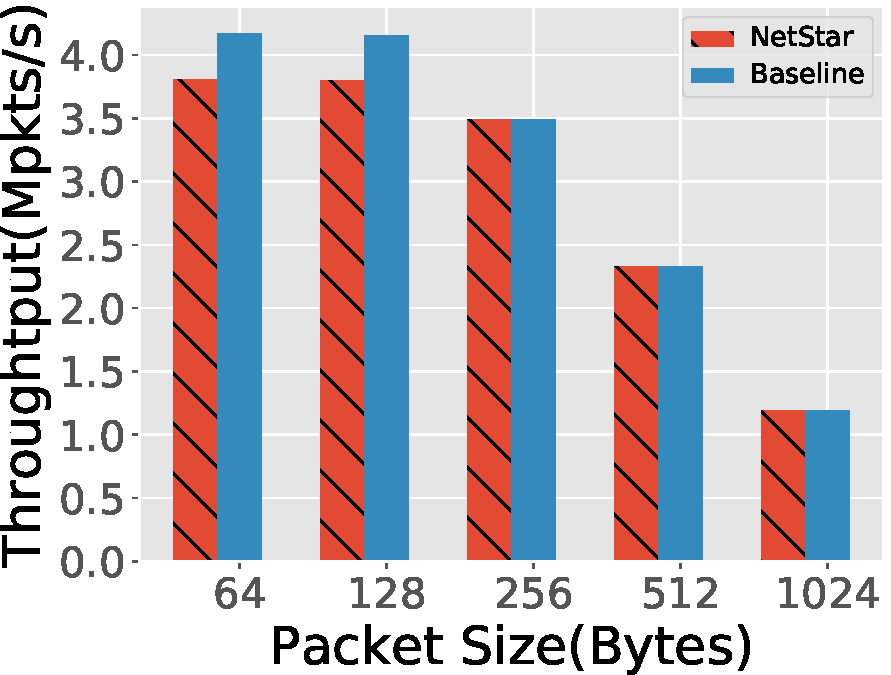
\includegraphics[width=\columnwidth]{chap-netstar/figure_src/Raw_forwarding_performance.pdf}
    \caption{}\label{fig:eval1.1}
  \end{subfigure}\hfill
  %\begin{subfigure}[t]{0.49\linewidth}
  %  \centering
  %  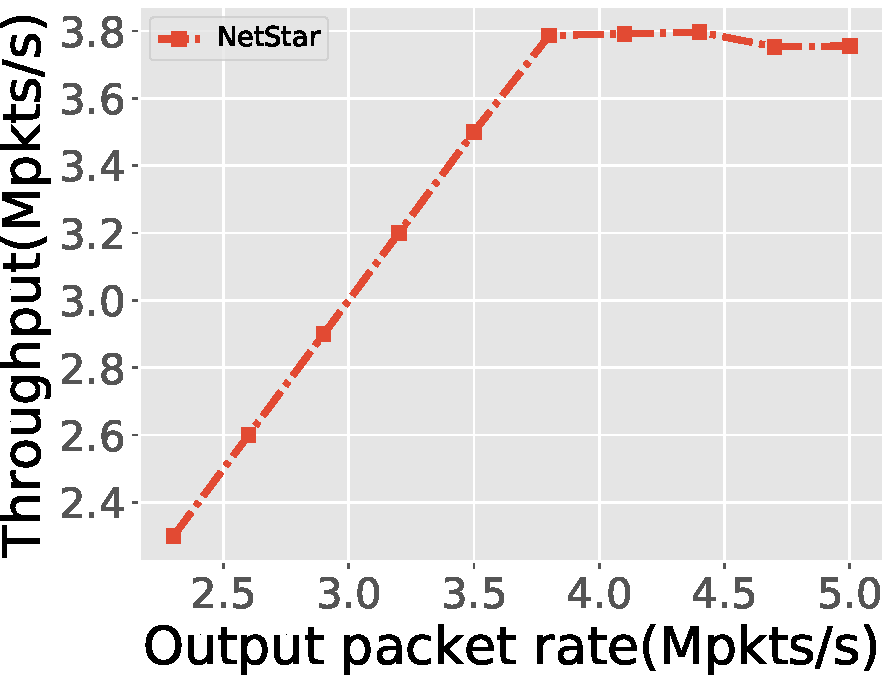
\includegraphics[width=\columnwidth]{figure_src/throughput_collapse.pdf}
  %  \caption{}\label{fig:eval1.2}
  %\end{subfigure}\hfill
  \begin{subfigure}[t]{0.49\linewidth}
    \centering
    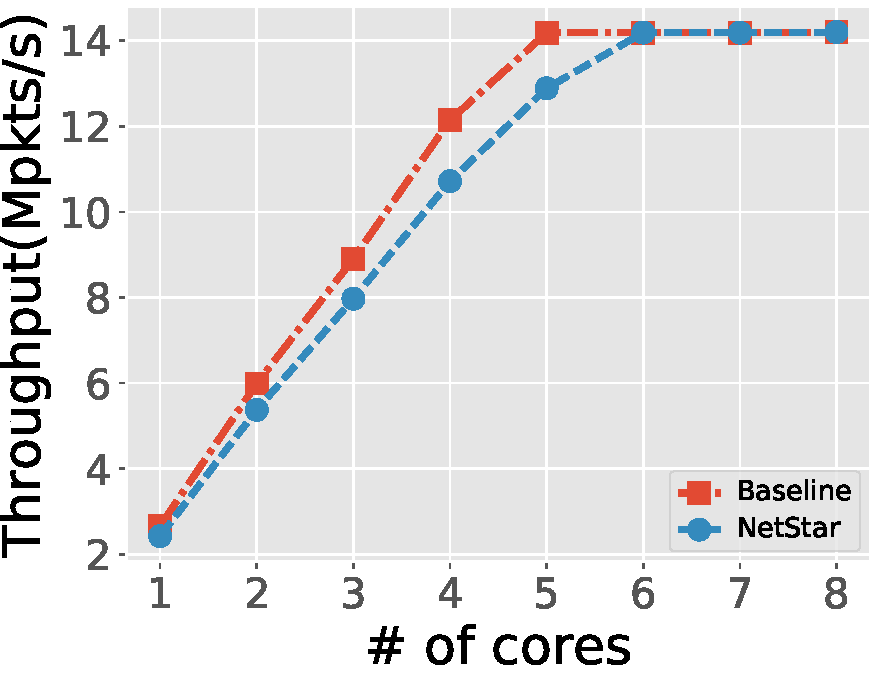
\includegraphics[width=\columnwidth]{chap-netstar/figure_src/scalability.pdf}
    \caption{}\label{fig:eval1.2}
  \end{subfigure}
\caption{Micro benchmarking on packet processing speed.}
\label{fig:eval1}
\end{figure}


To scale to line-rate processing when handling complex asynchronous operations, \netstar~should at least have adequate performance when being used as a simple packet forwarder. To evaluate this, we build a simple packet forwarder using \netstar, where the processing logic in each async-flow object is to directly forward all the received packets. For comparison, we also build a packet forwarder using DPDK \cite{dpdk}, which classifies packets into different flows by checking their flow-5-tuple against a cuckoo hash table adopted from the BESS virtual switch \cite{bess}, and passes packets belonging to a flow to its flow object for forwarding.
Compared with \netstar, the overhead associated with creating future object and chaining continuation functions are removed for the baseline forwarder, making it run faster. %To verify the effectiveness of our packet copy elimination optimization in Sec.~\ref{implementation}, we also show performance of a \netstar~version where fast packet optimization is disabled and the default Seastar handling is used.


Fig.~\ref{fig:eval1.1} shows packet processing throughput when the NFs are running on a single thread. 10000 UDP flows with different packet sizes are dispatched to an NF at the rate that is slightly larger than the maximum throughput achieved by the NF.
The throughput achieved by \netstar~is very close to the baseline. % when our optimization is in place. %Fig.~\ref{fig:eval1.1} also demonstrates the effectiveness of our fast packet optimization. We get an averaged 29\% throughput improvement over the unoptimized version.
%Fig.~\ref{fig:eval1.2} further shows the effectiveness of adopting our packet copy elimination in \netstar, when 10000 UDP flows with 64-byte packets are injected to the NF at gradually increasing packet rates.
%The generated traffic is sent to both the \netstar forwarder running on a single CPU core and an unoptimized forwarder. We measure the output packet rate and illustrate the result in . Besides improved performance,
 %It also ensures a more stable throughput even when the NF becomes overloaded. %According to Fig.~\ref{fig:eval1.2}, the unoptimized forwarder experience a 6\% throughput drop when overloaded while forwarder with fast packet optimization only experiences a 1\% throughput drop.
When each NF runs on multiple threads (CPU cores) and 100000 UDP flows with 64-byte packets at 10Gbps line rate are injected, Fig.~\ref{fig:eval1.2} shows that the throughput of \netstar~is always close to the baseline. With 6 cores, \netstar~achieves 10Gbps line rate. % input traffic consisting of 64 bytes small packets.
We evaluate \netstar~using small packets to better understand its packet forwarding performance, since larger packets are easier to saturate the NIC bandwidth, making NIC a bottleneck rather than revealing any performance bottleneck in our framework. We believe that the throughput of \netstar~can easily scale up to 40Gbps when it runs on a multi-core server and handles larger input packets.

%The core logic of the \netstar~forwarder is implemented with 75 LoC, whereas the baseline requires 93 LoC.

\subsubsection{Asynchronous Database Query}
\label{microbenchmark_db}

\begin{figure}[!h]
  \begin{subfigure}[t]{0.49\linewidth}
    \centering
    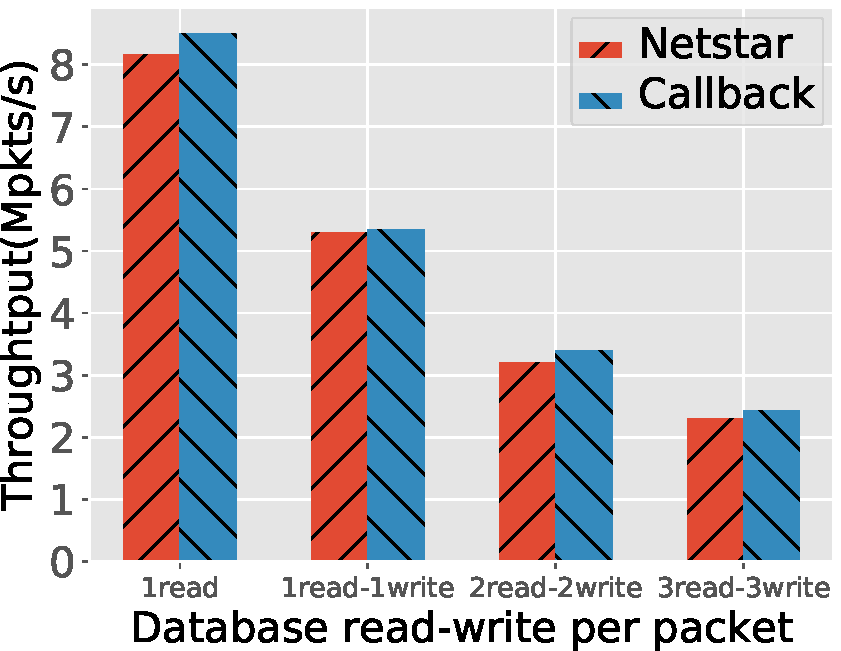
\includegraphics[width=\columnwidth]{chap-netstar/figure_src/read_write_throughput.pdf}
    \caption{}\label{fig:eval2.1}
  \end{subfigure}\hfill
  \begin{subfigure}[t]{0.49\linewidth}
    \centering
    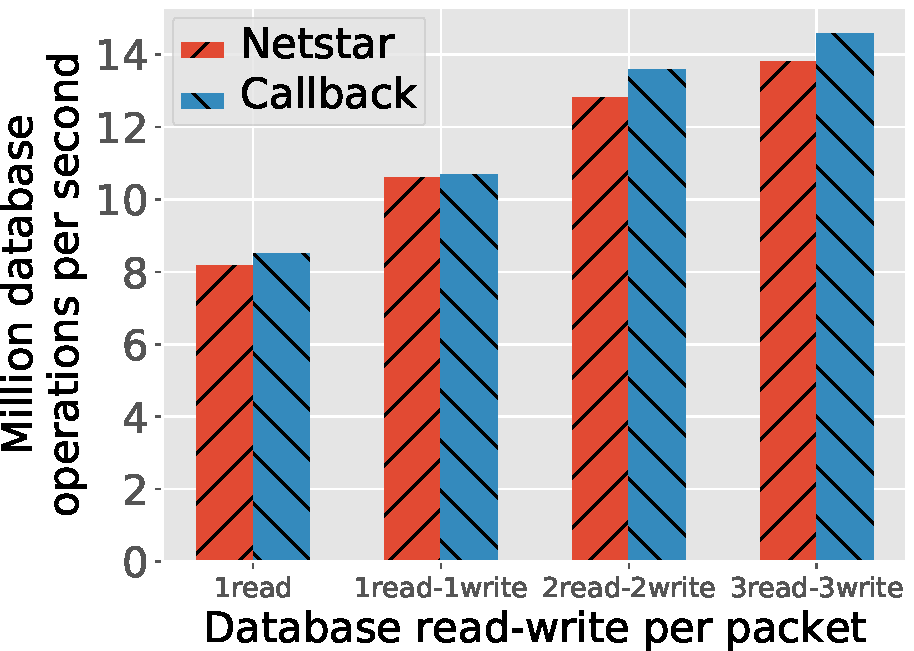
\includegraphics[width=\columnwidth]{chap-netstar/figure_src/read_write_speed.pdf}
    \caption{}\label{fig:eval2.2}
  \end{subfigure}
\caption{Micro benchmarking on asynchronous DB queries.}
\label{fig:eval2}
\end{figure}

We next develop a simple NF in which each async-flow object reads from and writes to a mica database as its core processing logic. Each write stores a key-value pair, where the key is the packet's flow-5-tuple and the value is a 24-byte random array. Each read retrieves a key-value pair using the packet's flow-5-tuple. We also implement the same NF functionality on a callback-based framework built on top of DPDK: a callback function is registered with each database query; when the database response arrives, the callback function is invoked to handle the response. Compared with the \netstar-based implementation, this framework imposes minimum runtime overhead when executing asynchronous operations: the registered callback is simply a function pointer without any heap allocation, whereas dynamic allocation and deallocation of future/promise object on the heap are involved in a future/promise-based framework.

%we vary the number of database queries that the async-flow object carries out per packet: from one read only, to one read-write, up to three consecutive read-write.
%The async-flow object may read-write the database multiple times and it only releases the received packet out when all the database queries finish.

We use 100000 UDP flows with 64-byte small packets at 10Gbps line rate. We vary the number of database read/write carried out by the NF when processing each packet. After receiving each packet, those read/write operations are consecutively carried out, before sending the packet out. Both \netstar~and the callback implementation run using 10 threads.
Fig~\ref{fig:eval2} shows that the packet processing throughput and the number of database queries that \netstar~can achieve is very close to that of the callback-based implementation. The average performance gap under various database access patterns is 4.23\% for packet throughput and 3.98\% for database operations per second.

%The core logic of the \netstar~implementation requires 54 LoC, whereas the baseline requires 80 LoC.
%Fig.~\ref{fig:eval2.2} shows that the \netstar can gradually increase the database query frequency if more database accesses are carried out for each processed packet. When the database is queries for 6 times to process a single packet, \netstar is capable of interacting with the database for over 13M times per second, while processing over 2M network packets.
%\chuan{give the LoC for each type of implementation}

\subsection{NFs from the StatelessNF paper\cite{201545}}
\label{sec:eval2}

\begin{figure}[!h]
  \begin{subfigure}[t]{0.49\linewidth}
    \centering
    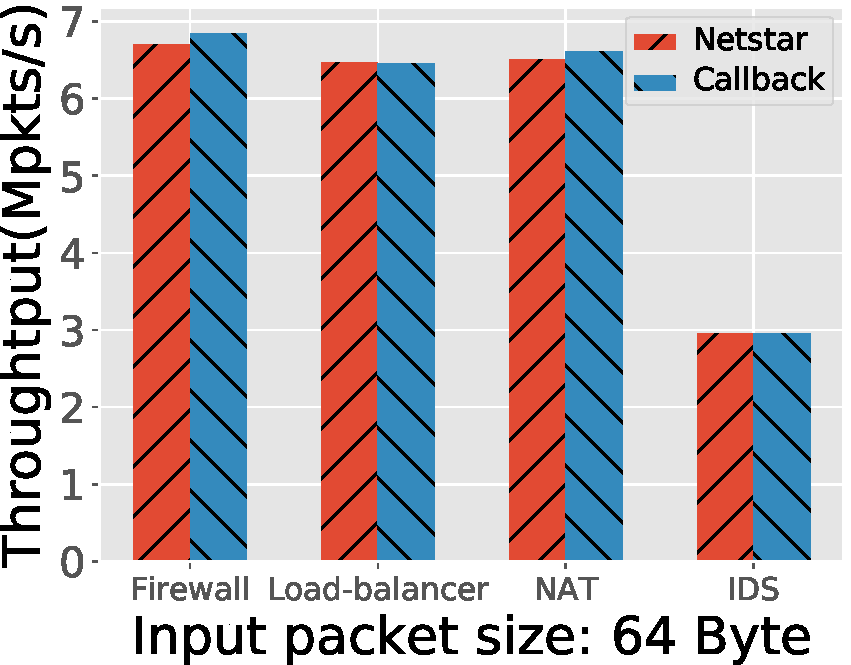
\includegraphics[width=\columnwidth]{chap-netstar/figure_src/StatelessNF_throughput_comparison_64byte.pdf}
    \caption{}\label{fig:eval3.1}
  \end{subfigure}\hfill
  \begin{subfigure}[t]{0.49\linewidth}
    \centering
    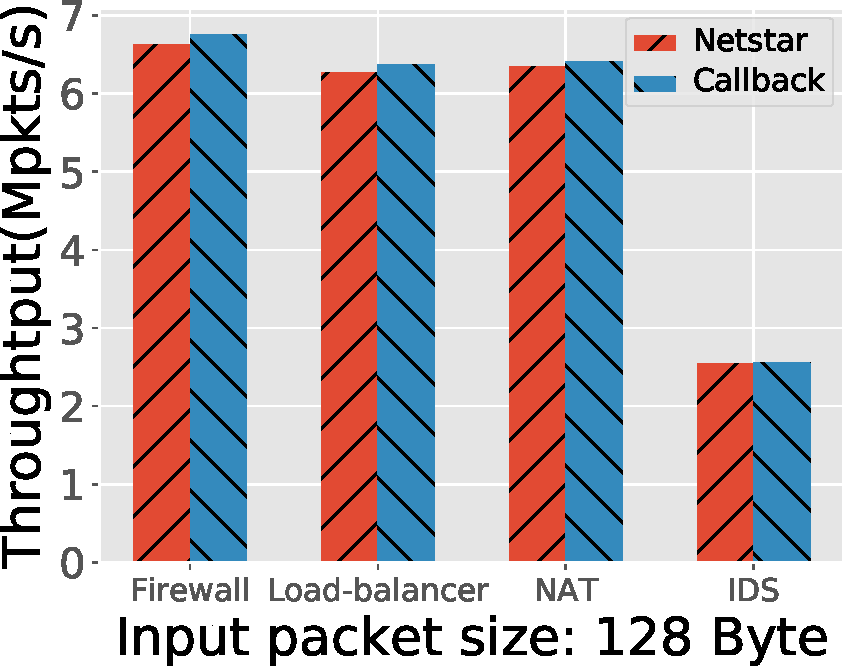
\includegraphics[width=\columnwidth]{chap-netstar/figure_src/StatelessNF_throughput_comparison_128byte.pdf}
    \caption{}\label{fig:eval3.2}
  \end{subfigure}\hfill
  \begin{subfigure}[t]{0.49\linewidth}
    \centering
    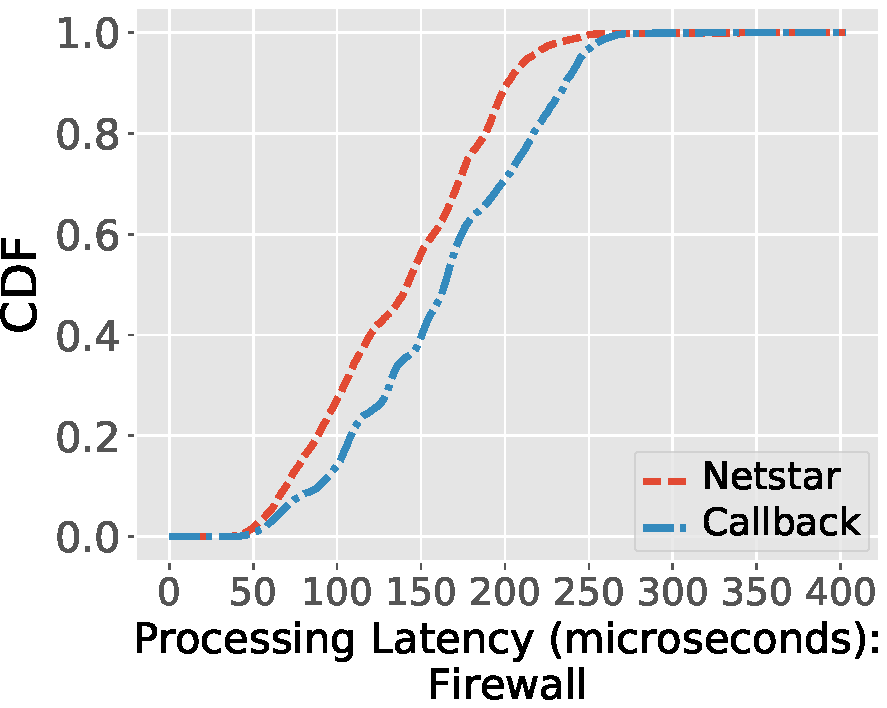
\includegraphics[width=\columnwidth]{chap-netstar/figure_src/firewall_throughput_latency_cdf.pdf}
    \caption{}\label{fig:eval3.3}
  \end{subfigure}\hfill
  \begin{subfigure}[t]{0.49\linewidth}
    \centering
    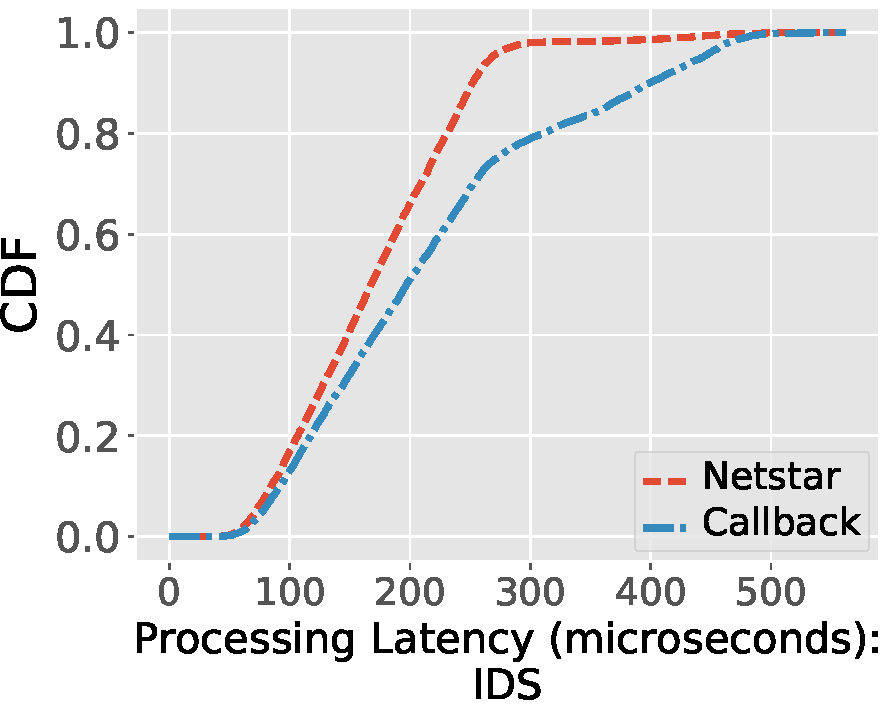
\includegraphics[width=\columnwidth]{chap-netstar/figure_src/ids_throughput_latency_cdf.pdf}
    \caption{}\label{fig:eval3.4}
  \end{subfigure}
\caption{Performance comparison: NFs from the StatelessNF paper.}
\label{fig:eval3}
\end{figure}


We compare our \netstar~based implementation of the four NFs with callback-based implementation (implemented following the pseudo-code logic), % using the callback-based framework as in Sec.~\ref{microbenchmark_db}),
as well as with the reported performance of NFs implemented by StatelessNF authors. We inject into each NF 100000 TCP flows at 10Gbps and vary the size of the flow packets. Each NF runs using 10 threads on a server, and accesses the mica database on a different server. % The NF reads and updates all the important per-flow state using the same procedure described in the StatelessNF paper.



%\noindent \textbf{A Callback-based Framework.}To evaluate the performance of \netstar framework, as well as comparing the implementation difficulty between future/promise abstraction and callback functions, we also implement the four NFs using a callback based framework. The callback based framework is implemented on top of DPDK for fast packet processing. To query mica database within this framework, the flow needs to register a callback function. When the database response arrives, the callback function is invoked to handle the response. Compared with \netstar, this framework imposes minimum runtime overhead when executing asynchronous operations: the registered callback function is simply a function pointer without any heap allocation, whereas future/promise abstraction needs to dynamically allocate and deallocate future/promise object on the heap.


In Fig.~\ref{fig:eval3.1} and Fig.~\ref{fig:eval3.2}, we observe that the packet processing throughput of our \netstar~NFs is very comparable with the callback-based NFs. % lower than 7M ppps for the firewall, NAT and load balancer. This is consistently with the evaluation result from Fig.~\ref{eval2.1}, as these three NFs only need to read the database once to process a single packet after the connection is established. The performance of IDS is smaller, due to the increased runtime overhead for passing the packet through AC automaton.
As compared to our observations in Sec.~\ref{microbenchmark_db}, when more complicated packet processing logic is involved here to process each packet besides executing asynchronous operations, the performance gap between \netstar~and the callback-based implementation decreases to only 2\%. We have also measured packet processing throughput when the packet size is 256, 512 or 1024 bytes. With a larger packet size, the NFs (except the IDS) can approach a 10Gbps processing rate. For IDS, the rate can reach 6.78 Gbps when processing 1024 bytes packets.

Fig.~\ref{fig:eval3.3} and Fig.~\ref{fig:eval3.4} show the CDF of packet processing latency at the firewall and the IDS when the packet size is 64 bytes. The packet processing latency between~\netstar~and the baseline is close to each other. %\netstar~achieves a smaller packet processing latency as the mica client library implemented in \netstar~has a more stable performance. %\chuan{give the reason}.

% We also compare throughout achieved by \netstar~NFs with reported performance in the StatelessNF paper. \netstar~can achieve over 6Mpps throughput on a single 10-core server (10 threads), while 4Mpps throughput is achieved in the paper using two 12-core servers.

%\subsubsection{Compare Implementation Difficulty.}

\begin{table}[!h]
\centering
\caption{LOC Comparison: NFs from the StatelessNF Paper}
\label{table:loc}
\resizebox{0.6\columnwidth}{!}{
\begin{tabular}{|l|l|l|l|}
\hline
   NF           & Callback  & \netstar  & Reduction \%\\ \hline
Firewall      & 52(44+8)  & 41(34+7) & 21.1\%        \\ \hline
Load balancer & 82(66+16) & 64(57+7) & 21.9\%        \\ \hline
NAT           & 99(79+20) & 80(73+7) & 19.1\%        \\ \hline
IDS           & 50(42+8)  & 43(36+7) & 14\%          \\ \hline
\end{tabular}
}
\vspace{-3mm}
\end{table}

To compare the implementation difficulty, we list the LOC for implementing the core processing logic of the four NFs using \netstar and the callback framework in Table~\ref{table:loc}. We only count the core processing code because a full-fledged implementation of each NF involves large volumes of auxiliary code on memory management, packet preprocessing and mica client library implementation. %All the four NFs require thousands lines of auxiliary code.
We can see that with the future/promise abstraction, the LOC can be reduced by as much as 21.9\%.
In the additions in Table~\ref{table:loc}, the number on the left is the total LOC for implementing packet processing functionalities, and the number on the right is the LOC for error handling. Due to consolidated error handling in \netstar, the same 7 lines of code are used for handling all errors in all NFs. %In the callback-based implementation,  requires defining redundant error handling logic in different callback functions. If the processing logic requires multiple asynchronous interactions with external services like the NAT, the redundant error handling logic may complicate the entire implementation.

\subsection{HTTP Reverse Proxy}
\label{sec:eval3}

\begin{figure}[!h]
  \begin{subfigure}[t]{0.49\linewidth}
    \centering
    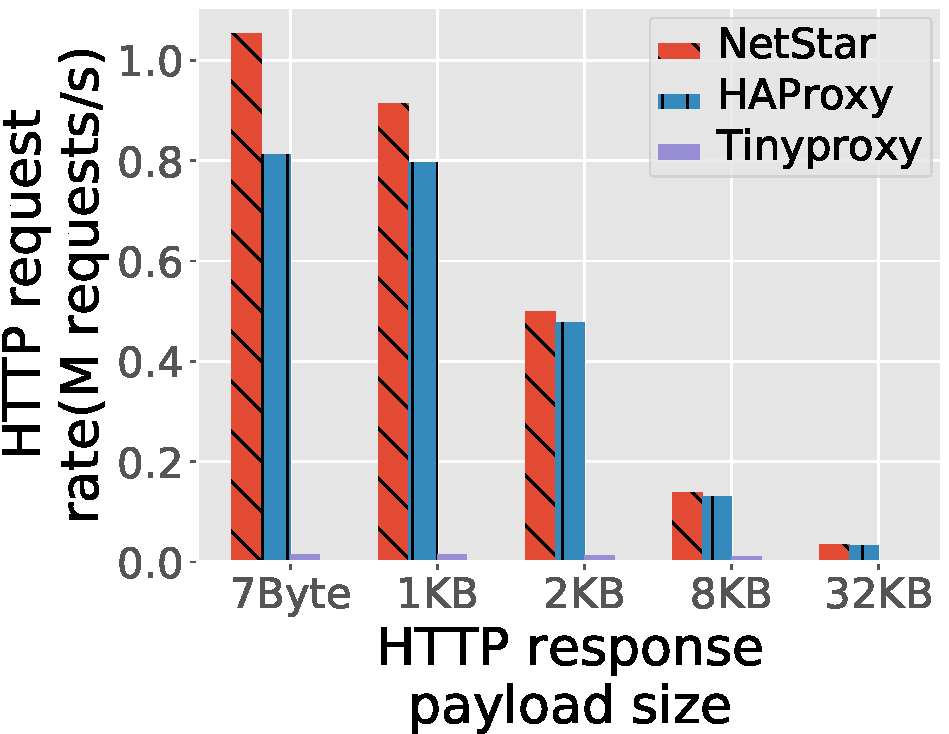
\includegraphics[width=\columnwidth]{chap-netstar/figure_src/Proxy_throughput.pdf}
    \caption{}\label{fig:eval4.1}
  \end{subfigure}\hfill
  \begin{subfigure}[t]{0.49\linewidth}
    \centering
    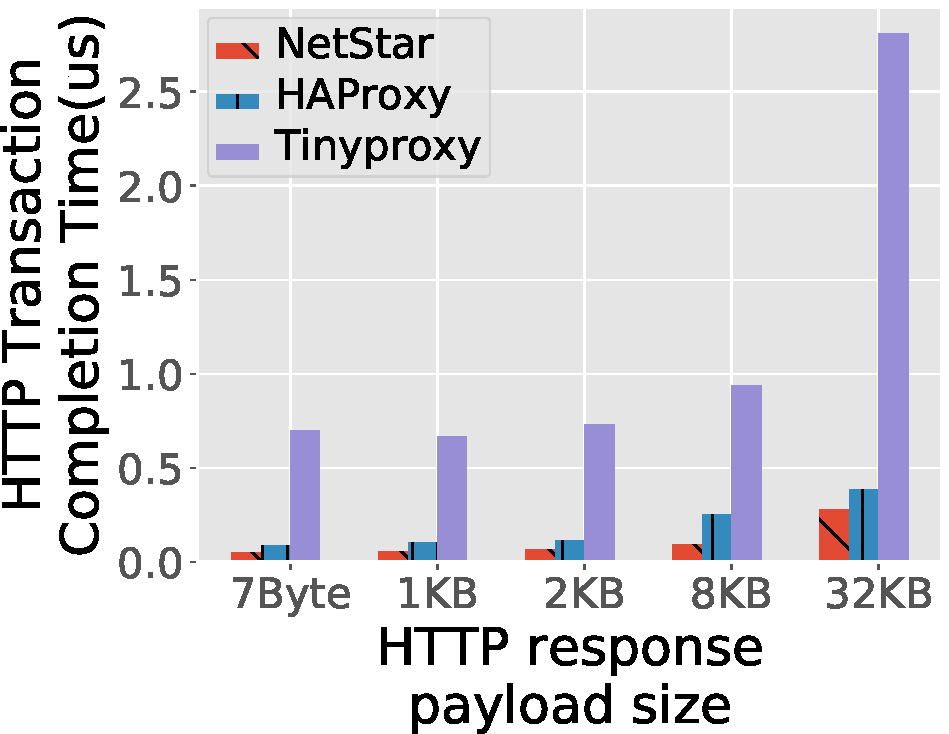
\includegraphics[width=\columnwidth]{chap-netstar/figure_src/Proxy_RTT.pdf}
    \caption{}\label{fig:eval4.2}
  \end{subfigure}
\caption{Performance comparison: different proxies.}%HTTP request rate and HTTP transaction completion time for different proxies.}
\label{fig:eval4}
\end{figure}


We compare our proxy implemented using \netstar~with both HAProxy version 1.8 \cite{haproxy} and TinyProxy version 1.8.4 \cite{tinyproxy}.
TinyProxy does not use a callback-based asynchronous design; instead, it creates a new thread to handle each TCP flow in a synchronous manner, and relies on the kernel scheduler to schedule different threads. Each proxy runs on 10 threads. %We configure all the proxies to fully utilize all the 10 CPU cores of the server.
We use the HTTP benchmarking tool to generate 200 connections that go through the proxy, and then keeps producing HTTP requests at the generator's maximal capability. %The payload size of HTTP responses varies from 7 bytes to 32K bytes. %The HTTP request rate and the HTTP transaction completion time are both recorded.

In Fig.~\ref{fig:eval4.1}, we see that \netstar~out-performs HAProxy by up to 20\% and is better than TinyProxy much more. As the payload size of HTTP response increases, the consumed bandwidth on the NIC gradually reaches 10Gbps, making the NIC a bottleneck and hence decreasing the performance gap. %When the size of the HTTP response content is 7 bytes, \netstar out-perform HAProxy by almost 20\%. The performance difference gradually diminishes as the size of the HTTP response content increases.
Fig.~\ref{fig:eval4.2} shows that the smallest HTTP transaction completion time is achieved by \netstar.

Note that we implement our proxy by translating the processing logic in TinyProxy, as our future/promise based framework can easily mimic a synchronous execution flow. Such a translated \netstar~proxy is easy to implement, runs in full asynchrony and has superior performance even compared to HAProxy, as shown by the above results.

%\chuan{give LOC results of the three proxies} HAProxy and TinyProxy are open-source software, we didn't implement them, so it's better not to compare the LoC.

\subsection {IDS}
\label{sec:eval4}

\begin{figure}[!h]
  \begin{subfigure}[t]{0.45\linewidth}
    \centering
    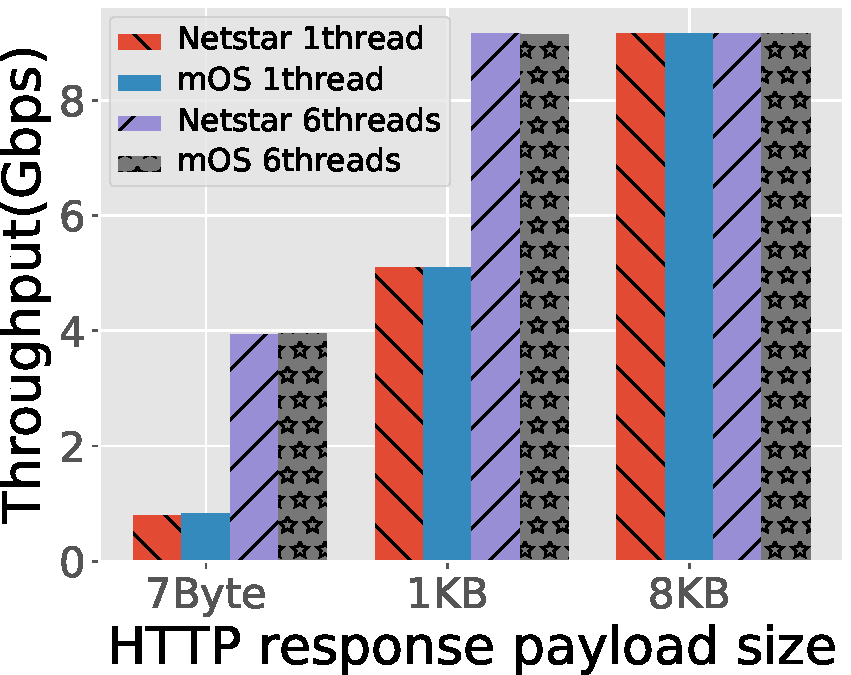
\includegraphics[width=\columnwidth]{chap-netstar/figure_src/IDS_throughput.pdf}
    \caption{}\label{fig:eval5.1}
  \end{subfigure}\hfill
  \begin{subfigure}[t]{0.53\linewidth}
    \centering
    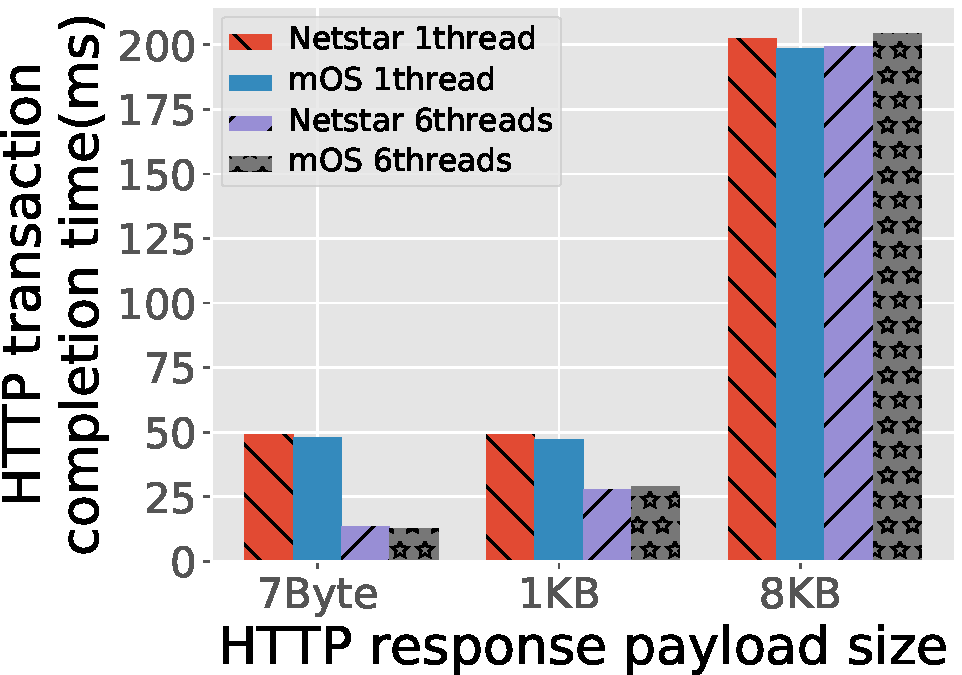
\includegraphics[width=\columnwidth]{chap-netstar/figure_src/IDS_RTT.pdf}
    \caption{}\label{fig:eval5.2}
  \end{subfigure}
\caption{Performance comparison: IDS.} %HTTP request rate and HTTP transaction completion time for IDSes implemented using \netstar and mOS.}
\label{fig:eval5}
\end{figure}

%\chuan{Fig.~\ref{fig:eval5}: change `HTTP response content size' to `HTTP response payload size'}

% To compare the performance of this IDS, we re-implement a similar IDS with mOS library \cite{}. We choose mOS because it is the state-of-art library implemented with callback-based event-driven style. We can use an implementation in mOS to evaluate whether NetStar approaches state-of-art performance.

We compare the IDS built with \netstar~and one built with mOS \cite{201546}, one of the fastest frameworks for building middleboxes that handle application-level payload reconstruction. mOS extensively uses the callback-based event-driven model. Our IDS implementation on mOS relies on registering various callback functions to the mOS framework to obtain reconstructed TCP byte stream and parsing HTTP request.
We generate 24K concurrent HTTP connections to pass through each IDS. %, then we measure the throughput and the HTTP transaction completion time achieved by the two IDSes.
The number of threads used by each IDSes varies, from 1 thread to 6 threads, to test the scalability.

In Fig.~\ref{fig:eval5}, we can see that the performance of \netstar~is very close to that achieved by the mOS-based implementation. %The highlight of \netstar is that the high-level programming environment it provides simplifies HTTP request parsing: after receiving a new piece of payload, we can convert the payload into an input stream and feed the input stream to an HTTP request parser provided in the Seastar framework, which is built with the REGAL library \cite{} and is robust to various parsing errors; then we can query from the parser whether we have received a complete HTTP request, and forward the entire HTTP request to the AC automaton for parsing. On contrary, the default HTTP request parser provided by mOS source code is rather simple. It only tries to inspect whether there contains special delimiter. This makes the HTTP request parser vulnerable to various parsing errors.
On the other hand, 493 LOC are written to implement the core processing logic in our \netstar~IDS, whereas 689 LOC are used in the mOS-based implementation, achieving a 28\% reduction.

\subsection {Malware Detector}
\label{sec:eval5}

\begin{table}[!h]
\centering
\caption{Performance of Malware Detectors}
\label{table:malware-detector-stat}
\resizebox{\columnwidth}{!}{
\begin{tabular}{|l|l|l|l|l|}
\hline
     & \begin{tabular}[c]{@{}l@{}}Throughput\\ (file size: 8k) \end{tabular} & \begin{tabular}[c]{@{}l@{}}Throughput\\ (file size: 32k) \end{tabular} & \begin{tabular}[c]{@{}l@{}}HTTP transaction\\ completion time \\(file size: 8k) \end{tabular} & \begin{tabular}[c]{@{}l@{}}HTTP transaction\\ completion time \\(file size: 32k) \end{tabular} \\ \hline
\begin{tabular}[c]{@{}l@{}}Asynchronous \\ Malware Detector\end{tabular} & 5.02 Gbps                                                              & 6.19 Gbps                                                                & 12.74 ms                                                                                    & 41.33 ms                                                                                     \\ \hline
\begin{tabular}[c]{@{}l@{}}Local Malware\\ Detector\end{tabular}         & 5.86 Gbps                                                               & 6.79 Gbps                                                                & 10.77 ms                                                                                   & 37.84 ms                                                                                     \\ \hline
\end{tabular}
}
\vspace{-5mm}
\end{table}

We compare our asynchronous malware detector that queries an external database and a DNS server (run in the same cluster as the malware detector) with a local malware detector that only tries to identify if the file hash exists in a local in-memory malware hash table. Both malware detectors are implemented using \netstar.
We generate 1000 HTTP connections and send files in these HTTP connections from the client to the server. We randomly populate the content of the file with malware. The size of the files vary from 8K bytes to 32K bytes. Both malware detectors run using one thread.% without multi-core scaling.

In Table~\ref{table:malware-detector-stat}, % shows the throughput and average HTTP transaction completion time achieved by both malware detectors.
 we can see that compared with a local version, the asynchronous malware detector experiences a 14\% throughput drop when the size of the transmitted file is 8K and 8.8\% throughput drop when the size of the transmitted file is 32K. The remote malware detection process adds a 1.97ms/3.48ms latency respectively. %Throughout the evaluation, all the generated malwares are successfully detected.

We purposely compare a malware detector accessing external services with a local malware detector, instead of a callback-based malware detector which also accesses external services, in order to show the following: our NF's performance is very comparable with a fast local detector, not to mention one accessing external services; with \netstar, complicated asynchronous operations can be enabled on NFs without large performance drop, and the future/promise abstraction provided by \netstar~enables easy implementation of the asynchronous operations.

\subsection{Comparison with Coroutine}
\label{sec:eval6}

Finally, we compare \netstar~with a coroutine based NF framework. %For \netstar, we reuse the NFs for querying the database as shown in~Sec.~\ref{}.
In the coroutine framework, for each new flow, a new coroutine (thread) is created and a similar packet processing loop as in our async-flow object runs within the coroutine. Whenever a coroutine needs to waits for an asynchronous event, it yields its control to other coroutines in the NF. %We directly utilize the coroutine module in Seastar to implement the coroutine framework.

We compare the \netstar~NF carrying out database queries in Sec.~\ref{microbenchmark_db} with a coroutine based implementation. 10000 UDP flows are sent to the two NFs, both running in one thread. Each NF reads the database once when processing one packet. A 750K pps throughput is achieved by the NF implemented with \netstar, while the throughput of the coroutine-based NF is only 147K pps. Further profiling reveals that the average coroutine switching time is around 352 nanoseconds. Even though the time is small, constant coroutine switching adds considerable overhead when an NF processes a large number of flows. %The constant coroutine switching adds considerable overheads to packet processing.
Therefore, coroutine is a less desirable paradigm for implementing asynchronous NFs when compared with the future/promise abstraction.
